% ----------------------------------------
% Chap: Konstruktive Bearbeitung
% ----------------------------------------
\chapter{Konstruktive Bearbeitung}
\label{chap:konstruktive_bearbeitung}

Um die Messgenauigkeit der optischen Interferometrie-Technik mit der einfachen Adaptierbarkeit an verschiedenen realen Maschinenelementen der elektrischen Messmethode zur Schmierfilmdickenmessung im EHD-Kontakt zu vereinigen, soll ein neues modulares Messsystem auf Basis des EHD-Prüfstands von PCS entwickelt werden.
Dieses System soll gleichzeitig die optische und elektrische (kapazitive) Messung erlauben.
Für ein solches System gibt es folgende Anforderungen, die durch konstruktive Bearbeitung in den nächsten Abschnitten gelöst werden:

% ----------------------------------------
% Itemize: Liste der konstruktiven Bearbeitungen
% ----------------------------------------
\begin{itemize}
    \item Elektrische Isolierung der Glasscheibe und der Kugel des gesamten Systems
    \item Elektrische Zugänge für die Messproben an der Scheibe und der Kugel
    \item Beschichtung auf der Scheibe, die eine elektrische und eine optische Messung gleichzeitig erlaubt.
\end{itemize}

% ----------------------------------------
% Sec: Konstruktion der Kugelführung
% ----------------------------------------
\section{Konstruktion der Kugelführung}
\label{sec:konstruktion_der_kugelfuehrung}

Da das modifizierte Kugelsupport mit einstellbarer Achse von \textit{E. Wittek}~\cite{wittek_2007} wegen Rundlaufabweichungen nur bis zu einer Wälzgeschwindigkeit von ca. \SI[per-mode=symbol]{0.7}{\meter\per\second} einsetzbar ist, wird die originale Kugelführung der Firma \textit{PCS Instruments} im Rahmen dieser Arbeit modifizierte und weiter benutzt.
Bei der standardmäßigen Kugelführung wird eine durchgebohrte Kugel in einem Adapter eingeklemmt, welche damit über einen Querstift mit der Motorausgangswelle des zweiten Antriebs formschlüssig verbunden wird.
Für die kapazitive Messung soll die Kugel elektrisch mit dem gesamten System isoliert werden.
Das erfolgt durch die Verwendung einer Kunststoffwelle.
Die Kugelaufnahme wird aus Messing gefertigt, um den Kontaktwiderstand der, das Signal übertragenden Kohlebürsten, zu reduzieren.
Abbildung~\ref{fig:aufbau_der_neuen_kugelfuehrung} zeigt den Zusammenbau der neuen Kugelführung an.

% ----------------------------------------
% Fig: Aufbau der neuen Kugelführung
% ----------------------------------------
\begin{figure}[htb]
    \centering
    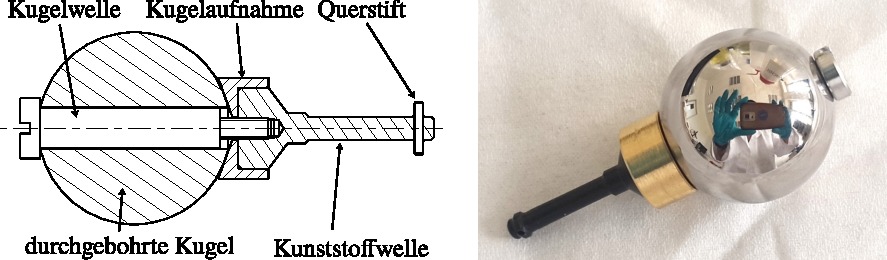
\includegraphics[]{./images/kugelfuehrung.pdf}
    \caption{Aufbau der neuen Kugelführung}
    \label{fig:aufbau_der_neuen_kugelfuehrung}
\end{figure}

Die geführte Kugelachse ermöglicht die Versuche mit Schlupf und verhindert auch das unkontrollierte Eindringen des Schmierstoffes (Öl, Fett) in den Kontakt.
Der Kraftfluss zwischen dem zweiten Motor und der Kugel kann durch den Wegfall des Querstifts unterbrochen werden.
In diesem Fall dreht sich die Kugelführung frei in der Motorausgangswelle.

% ----------------------------------------
% Sec: Konstruktion des Kugelsupports
% ----------------------------------------
\section{Konstruktion des Kugelsupports}
\label{sec:konstruktion_des_kugelsupports}

Das neue Kugelsupport besteht aus drei Rillenkugellagern, die durch drei M3 Schrauben auf einem dreieckigen Sockel befestigt werden (siehe Abbildung~\ref{fig:das_modifizierte_kugelsupport}).
Die Kugel wird von den drei Lagern sicher von unten gegen der Glasscheibe gedrückt.
Da die Kugel mit der Lasteinheit elektrisch isoliert werden muss, wird der Sockel aus Kunststoff gefertigt.
Auf der Unterseite des Sockels befinden sich zwei Löcher, die mit dem Stift der Lasteinheit arretiert werden, dadurch wird die Position des Kugelsupports während der Versuche sichergestellt.
An der Seite des Sockels sind zwei M3 Bohrung zur Anbringung der Kohlebürstenhalter, die für die Aufnahme der elektrischen Signale von der Kugel zuständig sind, versehen.
Bei den Versuchen mit Fett ist es dort auch möglich, die Befettungsvorrichtung zu montieren.

% ----------------------------------------
% Fig: Das modifizierte Kugelsupport
% ----------------------------------------
\begin{figure}[htb]
    \centering
    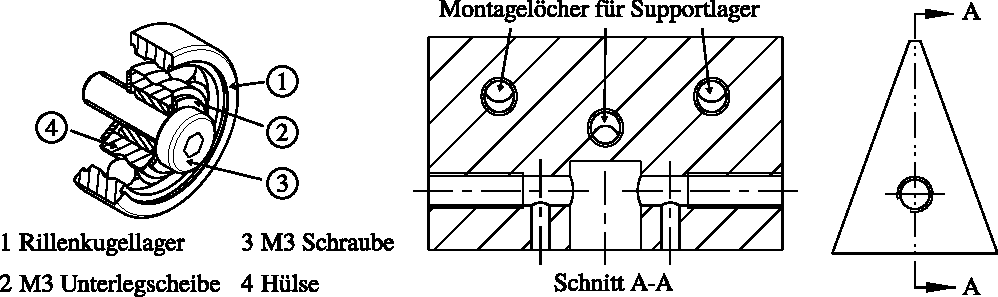
\includegraphics[]{./images/kugelsupport.pdf}
    \caption{Das Supportlager (links) und der Kunststoffsockel (rechts)}
    \label{fig:das_modifizierte_kugelsupport}
\end{figure}

Der Kohlebürstenhalter ist aus Messing, hat eine zylindrische Form und wird mit einem Blechhalter, welcher an der Seite des Supports angeschraubt wird, gelötet.
Die Kohlebürste Typ KK399 wurden von der Firma \textit{Schmidthammer} gekauft.
Dank dem hohen Kupferanteil (\SI{98}{\percent}) hat sie einen sehr geringen Kontaktwiderstand bzw. Eigenwiderstand.
Sie hat am Ende eine Kupferlitze und ist an der anderen Seite mit Laufschrägen versehen.
Leider sind die Laufschrägen für diese Anwendung nicht geeignet und wurden flach geschliffen.
Die Kohlebürste wird von einer Feder Typ LG860 gegen die Lauffläche der Kugelaufnahme gedrückt.
Abbildung~\ref{fig:die_baugruppe_des_kohlebuerstenhalters} zeigt die Baugruppe des Kohlebürstenhalters.

% ----------------------------------------
% Fig: Blechhalter + Kohlebürstenhalter + Kohlebürsten + Feder
% ----------------------------------------
\begin{figure}[htb]
    \centering
    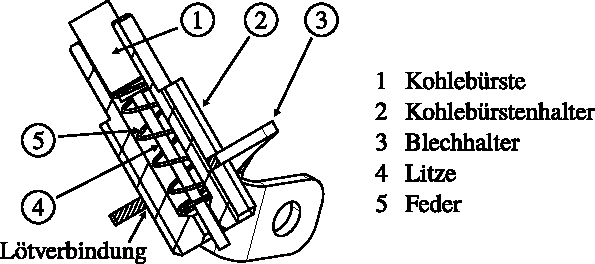
\includegraphics[]{./images/kohlebuerstenhalter_asm.pdf}
    \caption{Die Baugruppe des Kohlebürstenhalters}
    \label{fig:die_baugruppe_des_kohlebuerstenhalters}
\end{figure}

Um den elektrischen Kontakt zwischen der Kugel und der Messprobe während der Versuche gering an Störungen zu halten, sind zwei Kohlebürsten für die Kugel vorgesehen.
Abbildung~\ref{fig:das_komplette_kugelsupports} zeigt das komplette neue Support an.

% ----------------------------------------
% Fig: Zusammenbau des gesamten Kugelsupports
% ----------------------------------------
\begin{figure}[htb]
    \centering
    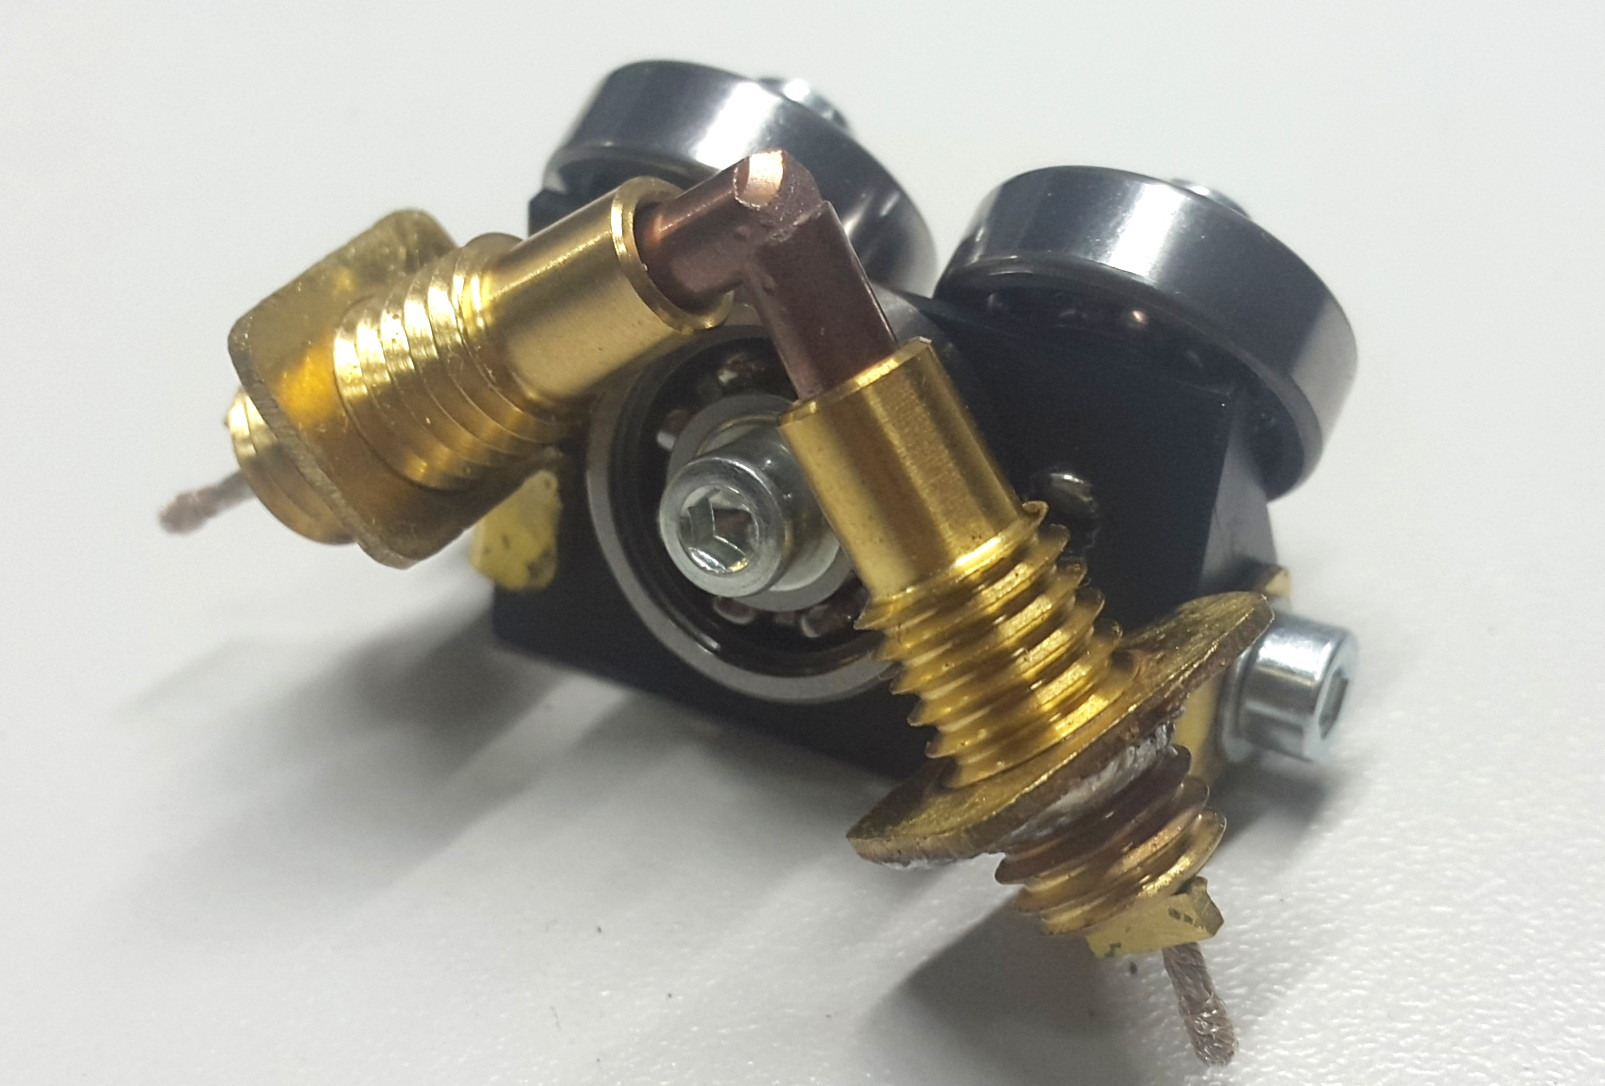
\includegraphics[width=0.5\linewidth]{./images/kugelsupport_full.jpg}
    \caption{Zusammenbau des neuen Kugelsupports}
    \label{fig:das_komplette_kugelsupports}
\end{figure}

% ----------------------------------------
% Sec: Die Glasscheibebaugruppe
% ----------------------------------------
\section{Die Glasscheibebaugruppe}
\label{sec:die_glasscheibebaugruppe}

Um die elektrische Messung bei dem vorhandenen Prüfstand durchzuführen, müssen die folgenden Maßnahmen durchgeführt werden:
% ----------------------------------------
% Itemize: Maßnahmen für die Glasscheibebaugruppe
% ----------------------------------------
\begin{itemize}
    \item Stromleitende Beschichtung für die Glasscheibe
    \item Isolierung der Glasscheibe mit dem gesamten Prüfsystem
    \item Elektrischer Zugang für die Messprobe zur Unterseite der Glasscheibe
\end{itemize}

Wie im vorherigen Kapitel~\ref{chap:literaturforschung_der_experimentellen_technik_in_ehd_schmierung} schon erwähnt, ist es auch möglich, die Schmierfilmdickenmessung bei einer Chrom-beschichteten Scheibe durchzuführen.
Allerdings gibt es folgende Probleme bei der klassischen Messmethode.
Erstens bietet dieses Verfahren eine niedrige Auflösung.
Zweitens ist eine monochrome Lichtquelle notwendig.
Es fehlt bei dem vorhandenen Prüfstand dieser Apparat.
Nicht zuletzt ist das \textit{Ultra-Softwarepaket} von \textit{PCS Instruments} nicht in der Lage, solche Messung durchzuführen bzw. auszuwerten.
Letztens ist der Eigenwiderstand der Chromschicht wegen der extrem dünnen Dicke sehr hoch (größer als \SI{1}{\kilo\ohm}).
Das macht die optische und elektrische Messung bei der Chrom-Glasscheibe ungünstig.

Eine andere Option ist es, die \textit{Spacer-Layer-Scheibe} zu benutzen.
Da die Silikatschicht nicht stromleitend ist, wird die Hälfte der Scheibe mit einer dickeren Chromschicht (c.a \SI{600}{\nano\meter}) beschichtet.
Durch die Erhöhung der Beschichtungsdicke wird der Eigenwiderstand reduziert.
Eine Widerstandsmessung mit dem Multimeter liefert den Wert von \SIrange{2.4}{8}{\ohm}.
Die neue Cr-Beschichtung weist eine Rauheit von $R_z =$ \SI{0.2}{\um}  auf und ist relativ glatt, so wie die Oberflächen des Herstellers (siehe Tabelle~\ref{fig:rauheitsmessung_ueber_der_risse} im Anhang).
Die Schmierfilmdicke kann wie normal mit dem EHD-Prüfstand von \textit{PCS} auf der unbehandelten Seite bestimmt werden.
Neben der neuen Glasscheibe wird auch eine Stahlscheibe gefertigt, um die kapazitive Messergebnisse mit der Glasscheibe zu kontrollieren.
Abbildung~\ref{fig:scheiben} zeigt die neue Glasscheibe mit der neuen Cr-Beschichtung (links) und die Stahlscheibe (rechts) an.

% ----------------------------------------
% Fig: Bild der neuen beschichteten Scheibe
% ----------------------------------------
\begin{figure}[htb]
    \centering
    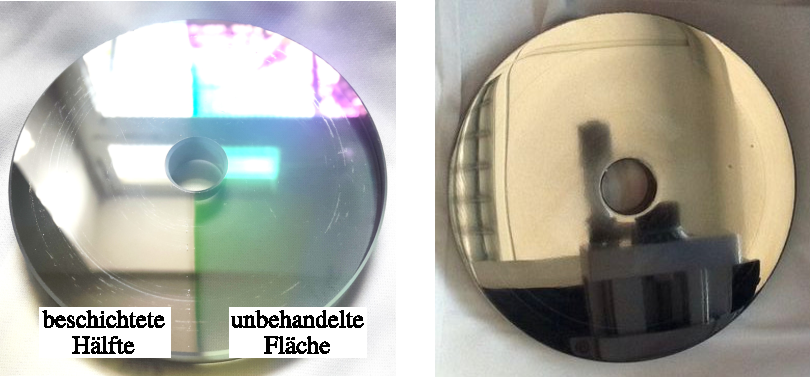
\includegraphics[]{./images/scheiben.pdf}
    \caption{Die neue Spacer-Layer-Glasscheibe mit sichbarer beschichteten Hälfte (links) und die Stahlscheibe (rechts)}
    \label{fig:scheiben}
\end{figure}

Der nächste Schritt ist, die behandelte Glasscheibe mit dem gesamten Testsystem zu isolieren.
Das erfolgt durch die Verwendung einer Kunststoff-Unterlegscheibe und einer Kunststoffhülse, die die Unterseite der Scheibe mit der Welle des ersten Motors trennen.
Beide Teile sind aus \textit{Polypropylen}, welches bis \SI{80}{\degreeCelsius} beständig ist.
Die Unterlegscheibe ist nur \SI{0.5}{\milli\meter} dick.
Da sich die Lasteinheit nicht nur in die horizontale sondern auch in die vertikale Richtung bewegen kann, ist diese minimale Höhenänderung der Glasscheibe kein Problem.
Die äußere Oberfläche der Hülse wurden an sechs Positionen flach gefräst.
Diese bilden mit der inneren Bohrung der Glasscheibe sechs Kanäle, die den Platz für die elektrische Verbindungen von Unterseite zur Oberseite der Scheibe schaffen.
Die Kunststoff-Unterlegscheibe wird mit der Hülse mit dem \textit{Plastix}-Kleber von Pattex verklebt.
Diese Verbindung ist gegen das Wegrutschen der beiden Teilen während Betriebs vorgenommen worden.
Abbildung~\ref{fig:isolierung_der_glassscheibe} zeigt die mit Kupferstreifen darauf befestigte Unterlegscheibe zur Isolierung der Glasscheibe und der ersten Motorwelle an.

% ----------------------------------------
% Fig: Isolierung der Scheibe
% ----------------------------------------
\begin{figure}[htb]
    \centering
    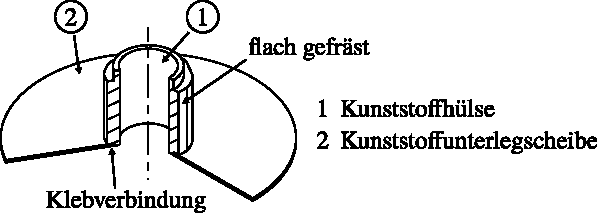
\includegraphics[]{./images/isolierung_der_scheibe.pdf}
    \caption{Isolierung der Glasscheibe}
    \label{fig:isolierung_der_glassscheibe}
\end{figure}

Um die elektrische Verbindung von der Unterseite der Scheibe nach oben zu bringen, werden sechs Kupferstreifen verwendet.
Sie werden auf der Kunststoff-Unterlegscheibe angeklebt und durch die sechs Kanäle (zwischen Hülse und Glasscheibe) nach oben geführt.
Dort werden sie bei der Montageposition zwischen die Oberkante der Hülse und eine Mitnehmerscheibe geklemmt.
Dadurch ist die elektrische Verbindung zwischen beiden Seiten der Scheibe hergestellt.
Die von oben geschraubte Sicherungsmutter sichert die gesamte Baugruppe fest.
Abbildung~\ref{fig:glasscheibebaugruppe} zeigt die ganze Baugruppe der Glasscheibe an.

% ----------------------------------------
% Fig: Glasscheibebaugruppe
% ----------------------------------------
\begin{figure}[htb]
    \centering
    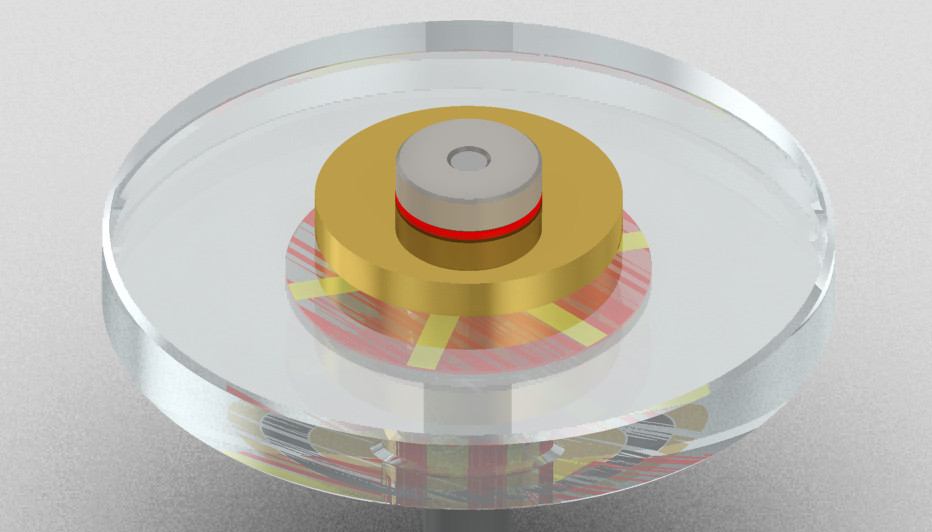
\includegraphics[width=0.7\linewidth]{./images/glasscheibe_asm.jpg}
    \caption{Die auf einer Testwelle montierte Glasscheibe und ihre dazu gehörigen Koponenten}
    \label{fig:glasscheibebaugruppe}
\end{figure}

% ----------------------------------------
% Sec: Konstruktion des Deckels
% ----------------------------------------
\section{Konstruktion des Deckels}
\label{sec:konstruktion_des_deckels}

Der originale Deckel des EHD-Prüfstands von PCS hat zwei wichtige Aufgaben:
Erstens soll er das Spritzöl vom Ölreservoir auf der Oberseite der Glasscheibe und in der Linsen der Lichtquelle verhindern.
Zweitens, da es nur eine Öffnung für die Lichtquelle auf dem Deckel gibt, soll er die Störungen, die durch Streulicht aus der Umgebung im EHD-Kontakt entstehen, bei der Messung reduzieren.

Für diese Arbeit wurde der Deckel modifiziert, so dass man die Kohlebürste, die das Messsignal von der Glasscheibe aufnimmt, in den Deckel integrieren kann.
Die gesamte Kohlebürste-Baugruppe wurde in dem Deckel durch eine M8 Bohrung angeschraubt und ihre Position durch eine Kontermutter gesichert.
Dadurch wird der elektrische Kontakt zwischen der Kohlebürste und der Glasscheibe über die Mitnehmerscheibe hergestellt.
An der Kante des Deckels gibt es eine kleine, gefräste Nut.
Durch diese werden die von der Kugel getragenen Messsignal-Leitungen nach draußen zu dem Messgerät geführt.
Abbildung~\ref{fig:deckel_mit_kohlebuersten} zeigt den neuen Deckel und den elektrischen Kontakt zwischen der im Deckel integrierten Kohlebürste und der Glasscheibe an.

% ----------------------------------------
% Fig: Der neue Deckel
% ----------------------------------------
\begin{figure}[htb]
    \centering
    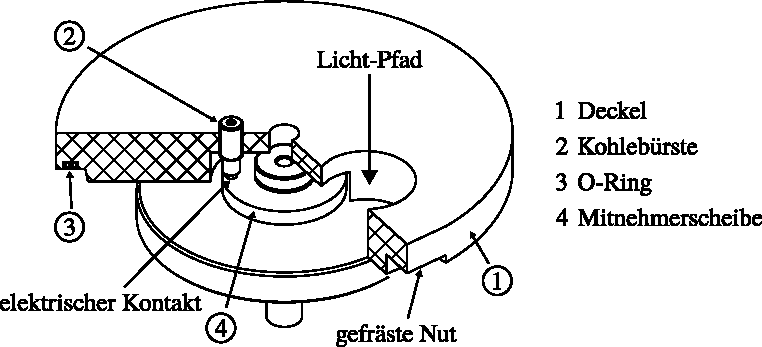
\includegraphics[]{./images/deckel_und_scheibe.pdf}
    \caption{Der neue Deckel mit der integrierten Kohlebürste}
    \label{fig:deckel_mit_kohlebuersten}
\end{figure}
